Jēdzientelpa ir vārdu vai frāžu attēlojums daudzdimensionālā vektoru telpā. Jēdzientelpas no teksta korpusa iegūst ar neironu tīkliem, kuri uztver kontekstu no tuvākajiem vārdiem tekstā. 

One hot encoding (vienizcēluma kodējums) dabiskās valodas apstrādē ir vektors, kurā katrs vektora elements ir sasaistīts ar vārdu krājuma elementu. Līdz ar to katrs vārds ir vektors, kurā atbilstošais elements ir 1 un visi pārējie elemeni ir 0. Piemēram, ja vārdu krājumā ir četri vārdi: karalis, karaliene, sieviete, vīrietis, karaliene tiktu kodēta kā [0, 1, 0, 0] \cite{colyer2016}.

Vektora garuma sasaiste ar vārdu krājuma izmēru ir trūkums, jo vārdu vektori ir cieši savienoti (coupled) ar korpusu un statiski, piemēram, pievienot jaunu vārdu nozīmē katram esošajam vārdu vektoram pievienot papildus nulli (nāktos pārtrennēt visu modeli(?)). Tāpat palielinoties dimensiju skaitam telpa pieaug tik strauji, ka daudzdimensiju telpām raksturīgs sparsity (neblīvums/izretinātība): one-hot encoding vektorā ir tikai viens nenulles elements un korpusos mēdz būt miljardiem vārdu. Visbeidzot one-hot encoding nesatur kontekstuālu vārdu nozīmi, nav korelācijas starp vārdiem ar līdzīgu nozīmi un lietojumu \cite{colyer2016}.


Atšķirībā no dabisko valodu apstrādes metodēm, kas katru vārdu uztver kā vienu atsevišķu vienību un tādēļ vienīgā iespējamā darbība ar vārdiem ir pārbaudīt vienādību, katras jēdzientelpas vektora vērtības ietekmē vārdi tiem apkārt jeb reprezentācija ir izkliedēta (distributed representation) un būtībā jēdzientelpas uztver attiecības starp vārdiem. Rezultātā vārdam atbilstošais vektors satur semantisku un sintaktisku informāciju par vārdu. No tā izriet praktiskā implikācija - ar vektoriem var darīt lineāro algebru - saskaitīt, atņemt utml \cite{colyer2016}.

Vārdus ir daudz grūtāk salīdzināt nekā skaitļus(, tādēļ mēs piešķiram vārdiem vektorus). Tomēr vārdi apraksta objektus ar noteiktām kvantificējamām īpašībām, piemēram, vieglāks/smagāks (masa), lētāks/dārgāks (cena). Šādai reprezentācijai ir jēga, jo dažādus objektus var salīdzināt savā starpā pēc īpašību vērtības jeb izteiktības pakāpes, piemēram, velosipēds ir vieglāks nekā mašīna. Tādā veidā vārda attēlojums tiek sadalīts pa visiem vektora elementiem, un katrs elements pievieno nozīmi daudziem vārdiem (\ref{fig:distributed-representation} attēls). Zinot, ka objektu īpašību skaitliska reprezentācija palīdz tos salīdzināt, atklājas jēga kvantitatīvi izteikt semantiku, tādējādi vārdi tiek attēloti veidā, kas izsaka to nozīmi (caur kontekstu). 

\begin{figure}[h]
	\centering
	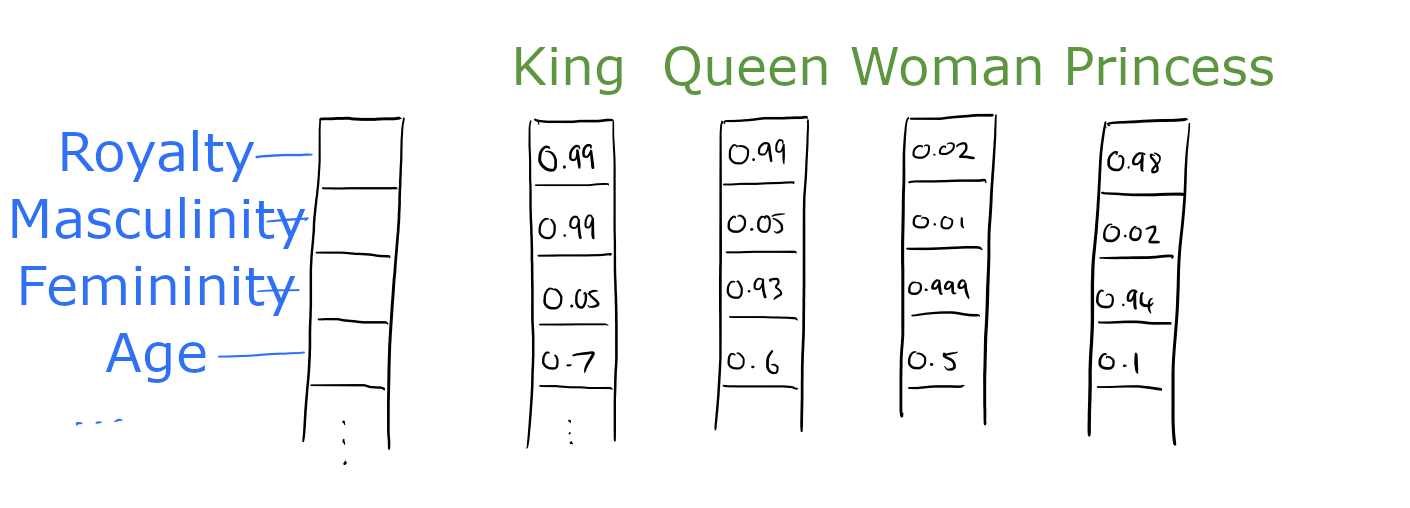
\includegraphics[width=\textwidth]{figures/word2vec-distributed-representation.png}
	\caption{Vārdu vektoru piemērs, kur katra dimensija ir novērtēta ar svariem un atbilst hipotētiskai vārda nozīmes niansei \cite{colyer2016}.}
	\label{fig:distributed-representation}
\end{figure}

Cilvēkiem uztverama jēdzientelpu analoģija ir krāsas nosaukums un tam atbilstošais vektors RGB krāsu modelī ar R, G un B koordinātēm no 0 līdz 255, piemēram, red = (255, 0, 0). Ar krāsu jēdzientelpām ir iespējams veikt saskaitīšanu un atņemšanu, kam ir fizikāla nozīme \cite{parrish2017}.

Atrast tuvākās krāsas sarkanam.
\begin{python}
closest(colors, colors['red'])
# red (229, 0, 0)
# fire engine red (254, 0, 2)
# bright red (255, 0, 13)
# tomato red (236, 45, 1)
# cherry red (247, 2, 42)
\end{python}

Operācijas ar vektoriem darbojas gan krāsu nosaukumiem semantiski, gan skaitliskiem vektoriem krāsu telpā. Piemēram, tuvākais vektors violeta un sarkana starpībai ir zils, kas atbilst cilvēku intuīcijai par RGB krāsām.
$$purple - red = blue$$
$$(126, 30, 156) - (229, 0, 0) = (-103, 30, 156)$$
\begin{python}
closest(colors, subtractv(colors['purple'], colors['red']))
# cobalt blue (3, 10, 167)
# royal blue (5, 4, 170)
# darkish blue (1, 65, 130)
# true blue (1, 15, 204)
# royal (12, 23, 147)
\end{python}

Tā saskaitot zaļu un zilu rodas kaut kas pa vidu - tirkīzs.
$$blue + green = turquoise$$
$$(3, 67, 223) + (21, 176, 26) = (24, 243, 249)$$
\begin{python}
closest(colors, addv(colors['blue'], colors['green']))
# bright turquoise (15, 254, 249)
# bright light blue (38, 247, 253)
# bright aqua (11, 249, 234)
# cyan (0, 255, 255)
# neon blue (4, 217, 255)
\end{python}

No vektoru operācijām var nolasīt secinājumus par semantiskajām attiecībām starp vārdiem, piemēram, rozā sarkanam ir tas pats, kas gaiši zils zilam.
$$pink - red + blue = light blue$$
$$(255, 129, 192) - (229, 0, 0) + (3, 67, 223) = (29, 196, 415)$$
\begin{python}
closest(colors, addv(subtractv(colors['pink'], colors['red']), colors['blue']))
# neon blue (4, 217, 255)
# bright sky blue (2, 204, 254)
# bright light blue (38, 247, 253)
# cyan (0, 255, 255)
# bright cyan (65, 253, 254)
\end{python}


Izrādās tādas pašas sakarības kādas ir krāsu nosaukumiem un to attēlojumiem krāsu telpā ir spēkā jebkuram vārdam (\ref{tab:semantic-relationship-examples} tabula). Vārdi, kuri bieži atrodas līdzīgos kontekstos, ir tuvāki nozīmē. Jēdzientelpas ietver gan sintaktiskas, gan semantiskas attiecības starp vārdiem. Jāuzsver, ka tādas semantiskas attiecības kā valsts-galvaspilsēta nav eksplicīti uzdotas, jēdzientelpu modelis tās ir novērojis tikai balstoties uz vārdu atrašanās vietām teksta korpusā. Iespēja trennēt modeli uz neanotētiem datiem kā šajā gadījumā samazina modeļa izmaksas valodām, kurās anotēti dati ir mazāk pieejami, un daudzkārt palielina potenciālās treniņu kopas apjomu, kas parasti ļauj sasniegt lielāku precizitāti.


Spēja noteikt sintaktisku un semantisku vārdu attiecības ir īpaši būtiska virtuālo asistentu jomā, jo, pirmkārt, semantiski līdzīgiem nodomiem ir līdzīgi vektori, tātad tie vienādi klasificēsies, otrkārt, informācija par sintakses attiecībām noder, jo lietotāji ievada jautājumus brīvā formā un tas ir it īpaši svarīgi fleksīvām valodām kā latviešu.



\begin{table}[htbp]
	\centering
	\caption{Semantisko attiecību piemēri}
	\begin{tabular}{ll}\toprule
		attiecība & piemērs  \\\midrule
		valsts-galvaspilsēta   & Parīze - Francija + Itālija = Roma \\
		valsts-valūta   & dolāri - ASV + Latvija = eiro \\
		vīrietis-sieviete   & karalis - vīrietis + sieviete = karaliene \\\bottomrule
	\end{tabular}%
	\label{tab:semantic-relationship-examples}%
\end{table}

\begin{table}[htbp]
	\centering
	\caption{Sintaktisko attiecību piemēri}
	\begin{tabular}{ll}\toprule
		attiecība & piemērs  \\\midrule
		daudzskaitlis   & pele - peles \\
		pagātne   & staigā - staigāja \\
		salīdzināmā pakāpe   & labs - labāks \\\bottomrule
	\end{tabular}%
	\label{tab:semantic-relationship-examples}%
\end{table}


\begin{figure}[h]
	\centering
	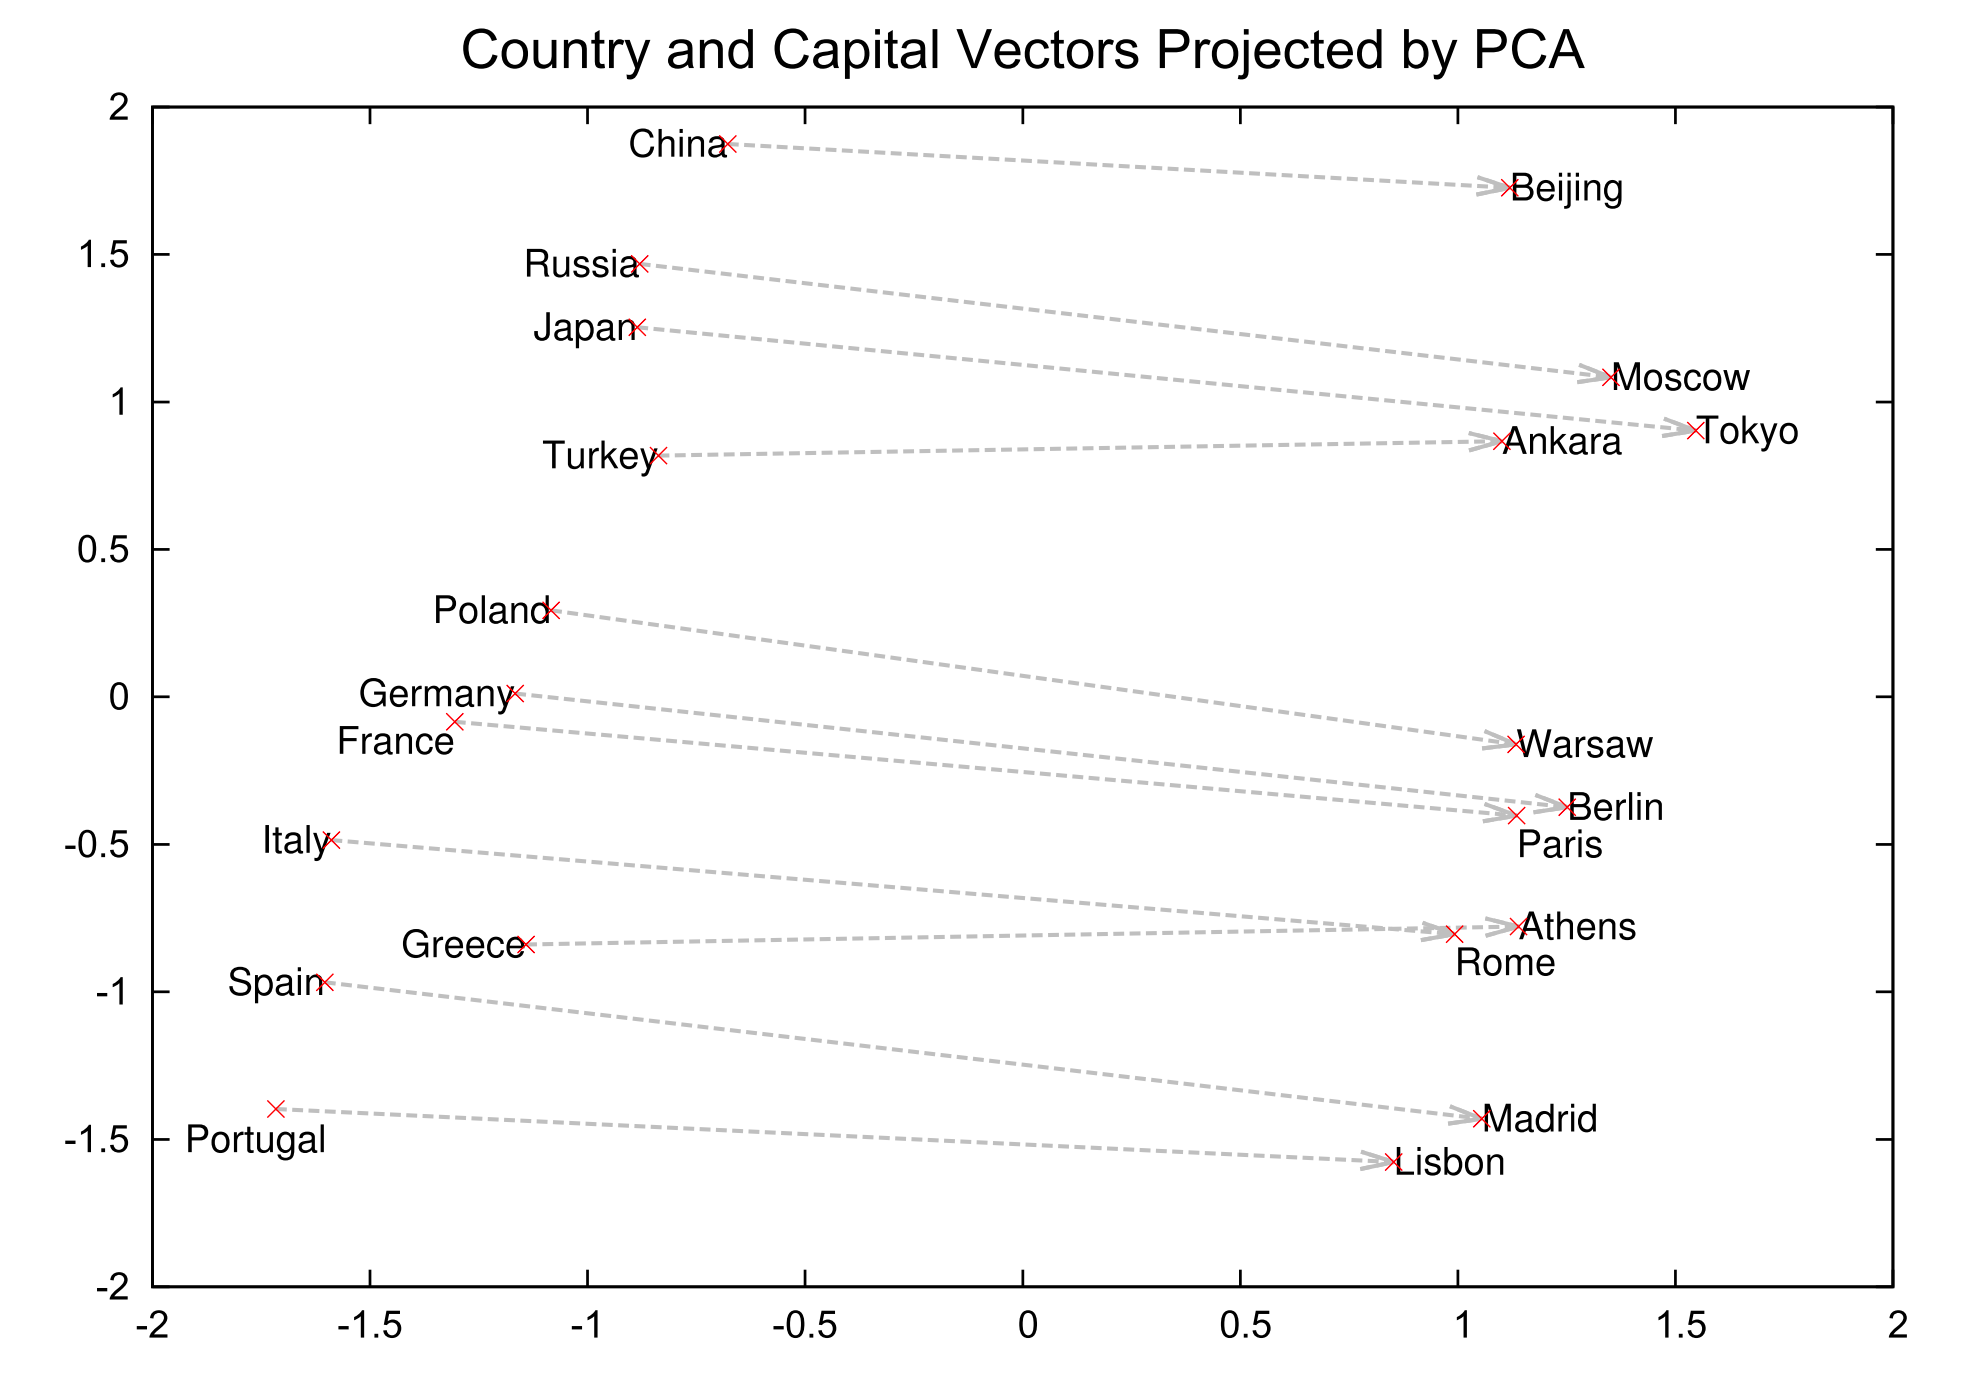
\includegraphics[width=\textwidth]{figures/word2vec-country-capital.png}
	\caption{Divdimensionāla PCA projekcija uzrāda attiecības starp valstu un galvaspilsētu jēdzientelpām}
\end{figure}

%distributed reprezentations
%http://www.cs.toronto.edu/~rgrosse/courses/csc321_2018/readings/L07%20Distributed%20Representations.pdf